\section{Kriging}\label{sec:kriging}

Gaussian process regression, also known as kriging \cite{bib:Matheron,bib:Rasmussen-regression,bib:GP-intro}, estimates the value of a field at an unobserved location using noisy measurements of the same field at known locations. Formally, let $f\sim\mathcal{GP}(m,k):\mathcal{U}\to\mathbb{R}^{d_z}$, and $x\in\mathcal{U}$. We wish to estimate the law of:
\begin{equation}
	z\triangleq f(x)+\varepsilon\in\mathbb{R}^{d_z},\qquad\varepsilon\sim\mathcal{N}(0,R),\qquad R\in\mathcal{S}_{d_z}^+(\mathbb{R})
\end{equation}

Without further information regarding $f$, we would only be able to state that $z$ follows a Gaussian distribution of expectation $m(x)$ and covariance $k(x,x)+R$. However, we are given $\tilde{n}\in\mathbb{N}^*$ distinct training points $\tilde{\mathbf{x}}\triangleq(\tilde{x}_1,\dots,\tilde{x}_{\tilde{n}})\in\mathcal{U}^{\tilde{n}}$ and their corresponding noisy observations:
\begin{equation}
	\tilde{\mathbf{z}}\triangleq\begin{bmatrix}
		f(\tilde{x}_1)+\varepsilon_1\\\vdots\\f(\tilde{x}_{\tilde{n}})+\varepsilon_{\tilde{n}}
	\end{bmatrix}\in\mathbb{R}^{\tilde{n}d_z},\qquad\varepsilon_i\sim\mathcal{N}(0,\tilde{R}),\qquad\tilde{R}\in\mathcal{S}_{d_z}^+(\mathbb{R})
\end{equation}
where the observation noises are also independent of $f$.

The goal of this section is to derive the best linear unbiased estimator (BLUE) of $z$ with respect to $\tilde{\mathbf{z}}$, \textit{i.e.} the estimator:
\begin{equation}
	\hat{z}=W^\top\tilde{\mathbf{z}}
\end{equation}
parametrised by a weight matrix:
\begin{equation}
	W\triangleq\begin{bmatrix}
	w_1\\\vdots\\w_{\tilde{n}}
	\end{bmatrix}\in\mathcal{M}_{\tilde{n}d_z,d_z}(\mathbb{R})
\end{equation}
such that the error vector has an expectation of $0$ and a minimum covariance.

Since $\hat{z}-z$ is a vector, its covariance is a matrix, and cannot be minimised as such. To alleviate this issue, we minimise its trace, which is exactly the mean squared error:
\begin{equation}
	\operatorname{tr}(\mathbb{V}[\hat{z}-z])=\mathbb{E}\left[\|\hat{z}-z\|^2\right]\label{eq:error_covariance}
\end{equation}

In the following, we present three kriging estimates, based on increasingly relaxed assumptions made on our knwoledge of the underlying GP. Each method relies on the inversion of the Gram matrix:
\begin{equation}
	\begin{aligned}
	G(\tilde{\mathbf{x}})&\triangleq k(\tilde{\mathbf{x}},\tilde{\mathbf{x}})+I_{\tilde{n}}\otimes\tilde{R}\\
	&=\begin{bmatrix}
	k(\tilde{x}_1,\tilde{x}_1)+\tilde{R}&\cdots&k(\tilde{x}_1,\tilde{x}_{\tilde{n}})\\\vdots&\ddots&\vdots\\k(\tilde{x}_{\tilde{n}},\tilde{x}_1)&\cdots&k(\tilde{x}_{\tilde{n}},\tilde{x}_{\tilde{n}})+\tilde{R}
	\end{bmatrix}
	\end{aligned}\label{eq:Gram_matrix}
\end{equation}
of $\tilde{\mathbf{x}}$ with respect to $f$, where $\otimes$ is the Kronecker matrix product. Since $k$ is SPD and the training points are distinct, it comes that:
\begin{equation}
	G(\tilde{\mathbf{x}})\in\mathcal{S}_{\tilde{n}d_z}^{++}(\mathbb{R})
\end{equation}
and so $G(\tilde{\mathbf{x}})$ is invertible, even in the noiseless case $\tilde{R}=0$.

We further assume that the query point $x$ differs from the training points $\tilde{\mathbf{x}}$, so that the joint law of $(z,\tilde{\mathbf{z}})$ is non-degenerate. This hypothesis is not restrictive and is only needed for the proofs. Indeed, the estimators are continuous in $x$ and thus remain valid at the training points as soon as $m$ and $k$ are continuous, which we assume.

\textbf{TODO: à reformuler} Whatever the weight matrix, $\mathbb{V}\left[\hat{z}-z\right]$ is a covariance matrix and is therefore SPSD. Non-degeneracy makes it SPD, as for $a\in\mathbb{R}^{d_z}\setminus\{0\}$, the vector $v\triangleq\begin{bmatrix}-a\\W\:a\end{bmatrix}\in\mathbb{R}^{d_z+\tilde{n}d_z}$ is non-zero and satisfies:
\begin{equation}
	a^\top\mathbb{V}\left[\hat{z}-z\right]a=\mathbb{V}\left[v^\top\begin{bmatrix}z\\\tilde{\mathbf{z}}\end{bmatrix}\right]=v^\top\mathbb{V}\left[\begin{bmatrix}z\\\tilde{\mathbf{z}}\end{bmatrix}\right]v>0\label{eq:kriging_covariance_SPD}
\end{equation}
Each covariance derived below is this quantity at a particular weight matrix, and inherits both properties.

\Cref{fig:kriging_example} illustrates this setting for a scalar field over a one-dimensional index set.

\begin{figure}[!htb]
	\centering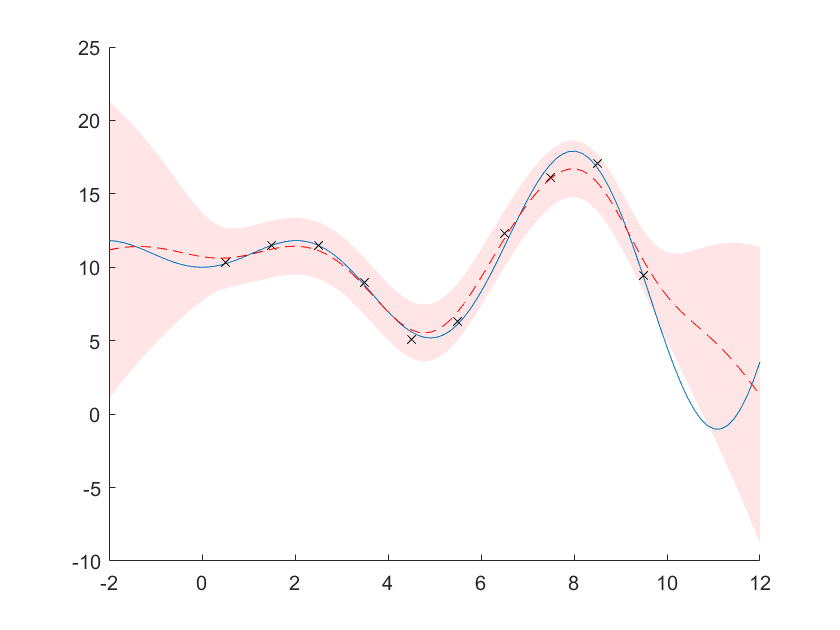
\includegraphics[width=0.7\textwidth]{../../Images/Exemple de krigeage 2D.png}
	\caption{Kriging of a scalar field from noisy samples. The estimate tracks the true field within the sampled region and departs from it outside, where the confidence band widens.}\label{fig:kriging_example}
\end{figure}

\subsection{Simple Kriging}

Simple kriging is the simplest form of kriging, and assumes that the mean function $m$ is known. \Cref{th:simple_kriging} gives a closed-form expression of the simple kriging estimator and its associated covariance matrix, while \Cref{th:simple_kriging_conditional} shows that it coincides with the conditional distribution of $z$ given $\tilde{\mathbf{z}}$.

\begin{proposition}[Simple kriging estimator]\label{th:simple_kriging}
	Using the notations introduced in \cref{sec:kriging}, the simple kriging estimator of $z$ and its error covariance are:
	\begin{equation}
		\left\{\begin{aligned}
		\hat{z}_{\mathrm{SK}}(x,\tilde{\mathbf{x}},\tilde{\mathbf{z}},m)&=m(x)+k(x,\tilde{\mathbf{x}})\:G(\tilde{\mathbf{x}})^{-1}\:(\tilde{\mathbf{z}}-m(\tilde{\mathbf{x}}))\\
		\hat{R}_{\mathrm{SK}}(x,\tilde{\mathbf{x}})&=k(x,x)+R-k(x,\tilde{\mathbf{x}})\:G(\tilde{\mathbf{x}})^{-1}k\left(\tilde{\mathbf{x}},x\right)
		\end{aligned}\right.\label{eq:simple_kriging_equations}
	\end{equation}
\end{proposition}

\begin{proof}
	Since $m$ is known, we may assume it to be identically equal to $0$ by working with $f-m$ instead of $f$, without any loss of generality. In the centred case, \eqref{eq:error_covariance} can be developed as follows:
	\begin{equation}
		\mathbb{V}[W^\top\tilde{\mathbf{z}}-z]=W^\top G(\tilde{\mathbf{x}})\:W-W^\top k(\tilde{\mathbf{x}},x)-k(x,\tilde{\mathbf{x}})\:W+k(x,x)+R\label{eq:generic_kriging_variance}
	\end{equation}

	By symmetry of $G(\tilde{\mathbf{x}})$, differentiating \eqref{eq:error_covariance} with respect to $W$ yields:
	\begin{equation}
		\begin{aligned}
		&\frac{\partial}{\partial W}\left(\operatorname{tr}\left(W^\top G(\tilde{\mathbf{x}})\:W-W^\top k(\tilde{\mathbf{x}},x)-k(x,\tilde{\mathbf{x}})\:W+k(x,x)+R\right)\right)=0\\
		\iff\quad&\frac{\partial}{\partial W}\left(\operatorname{tr}\left(W^\top G(\tilde{\mathbf{x}})\:W\right)\right)-2\frac{\partial}{\partial W}\left(\operatorname{tr}\left(W^\top k(\tilde{\mathbf{x}},x)\right)\right)=0\\
		\iff\quad&2G(\tilde{\mathbf{x}})\:W-2k(\tilde{\mathbf{x}},x)=0\\
		\iff\quad&W=G(\tilde{\mathbf{x}})^{-1}k(\tilde{\mathbf{x}},x)
		\end{aligned}
	\end{equation}

	The simple kriging estimator is thus:
	\begin{equation}
		\hat{z}_{\mathrm{SK}}=W^\top\tilde{\mathbf{z}}=k(x,\tilde{\mathbf{x}})\:G(\tilde{\mathbf{x}})^{-1}\tilde{\mathbf{z}}
	\end{equation}
	and its corresponding covariance:
	\begin{equation}
		\begin{aligned}
		\hat{R}_{\mathrm{SK}}&=W^\top G(\tilde{\mathbf{x}})\:W-W^\top k(\tilde{\mathbf{x}},x)-k(x,\tilde{\mathbf{x}})\:W+k(x,x)+R\\
		&=k(x,\tilde{\mathbf{x}})\:G(\tilde{\mathbf{x}})^{-1}G(\tilde{\mathbf{x}})\:G(\tilde{\mathbf{x}})^{-1}k(\tilde{\mathbf{x}},x)-k(x,\tilde{\mathbf{x}})\:G(\tilde{\mathbf{x}})^{-1}k(\tilde{\mathbf{x}},x)\\
		&\qquad-k(x,\tilde{\mathbf{x}})\:G(\tilde{\mathbf{x}})^{-1}k(\tilde{\mathbf{x}},x)+k(x,x)+R\\
		&=k(x,x)+R-k(x,\tilde{\mathbf{x}})\:G(\tilde{\mathbf{x}})^{-1}k(\tilde{\mathbf{x}},x)
		\end{aligned}
	\end{equation}

	The general case is obtained by adding $m$ back into $f$.
\end{proof}

\begin{remark}[Error covariance minimisation]
	While the simple kriging weights $W=G^{-1}k(\tilde{\mathbf{x}},x)$ were obtained by minimising the trace of $\mathbb{V}[\hat{z}-z]$, they actually minimise the whole covariance in the SPSD sense. Indeed:
	\begin{equation}
		\begin{aligned}
		\mathbb{V}[\hat{z}-z]-\hat{R}_{\mathrm{SK}}&=W^\top G(\tilde{\mathbf{x}})\:W-W^\top k(\tilde{\mathbf{x}},x)-k(x,\tilde{\mathbf{x}})\:W+k(x,\tilde{\mathbf{x}})\:G(\tilde{\mathbf{x}})^{-1}k(\tilde{\mathbf{x}},x)\\
		&=\left(W-G(\tilde{\mathbf{x}})^{-1}k(\tilde{\mathbf{x}},x)\right)^\top G(\tilde{\mathbf{x}})\left(W-G(\tilde{\mathbf{x}})^{-1}k(\tilde{\mathbf{x}},x)\right)\\
		&\succeq0
		\end{aligned}
	\end{equation}
	with equality if and only if $W=G(\tilde{\mathbf{x}})^{-1}k(\tilde{\mathbf{x}},x)$ since $G(\tilde{\mathbf{x}})\succ0$.
\end{remark}

\begin{proposition}[Exact interpolation in the noiseless case]
	Assume that $\tilde{R}=0$, and let $i\in[\![1,\tilde{n}]\!]$. The simple kriging estimator interpolates the data at $\tilde{x}_i$ exactly:
	\begin{equation}
		\left\{\begin{aligned}
		\hat{z}_{\mathrm{SK}}(\tilde{x}_i,\tilde{\mathbf{x}},\tilde{\mathbf{z}},m)&=\tilde{z}_i\\
		\hat{R}_{\mathrm{SK}}(\tilde{x}_i,\tilde{\mathbf{x}})&=R
		\end{aligned}\right.
	\end{equation}

	In particular, the error covariance reduces to the query noise $R$ alone, and vanishes when $R=0$. On the contrary, a positive training noise $\tilde{R}\succ0$ turns kriging into a smoother rather than an interpolator \cite{bib:spline-correspondence}.
\end{proposition}

\begin{proof}
	Since $\tilde{R}=0$, the Gram matrix reduces to $G(\tilde{\mathbf{x}})=k(\tilde{\mathbf{x}},\tilde{\mathbf{x}})$. Let $e_i\triangleq[0,\dots,0,1,0,\dots,0]^\top$ be the $i$-th canonical basis vector of $\mathbb{R}^{\tilde{n}}$. The matrix $e_i^\top\otimes I_{d_z}$ extracts the $i$-th block of a stacked matrix, such that:
	\begin{equation}
		\left(e_i^\top\otimes I_{d_z}\right)G(\tilde{\mathbf{x}})=\left(e_i^\top\otimes I_{d_z}\right)k(\tilde{\mathbf{x}},\tilde{\mathbf{x}})=k(\tilde{x}_i,\tilde{\mathbf{x}})
	\end{equation}

	The kriging weights thus reduce to this selector:
	\begin{equation}
		k(\tilde{x}_i,\tilde{\mathbf{x}})\:G(\tilde{\mathbf{x}})^{-1}=\left(e_i^\top\otimes I_{d_z}\right)G(\tilde{\mathbf{x}})\:G(\tilde{\mathbf{x}})^{-1}=e_i^\top\otimes I_{d_z}
	\end{equation}

	Evaluating \eqref{eq:simple_kriging_equations} at $x=\tilde{x}_i$ by the continuity yields:
	\begin{equation}
		\begin{aligned}
			\hat{z}_{\mathrm{SK}}(\tilde{x}_i,\tilde{\mathbf{x}},\tilde{\mathbf{z}},m)&=m(\tilde{x}_i)+k(\tilde{x}_i,\tilde{\mathbf{x}})\:G(\tilde{\mathbf{x}})^{-1}\left(\tilde{\mathbf{z}}-m(\tilde{\mathbf{x}})\right)\\
			&=m(\tilde{x}_i)+\left(e_i^\top\otimes I_{d_z}\right)\left(\tilde{\mathbf{z}}-m(\tilde{\mathbf{x}})\right)\\
			&=m(\tilde{x}_i)+\tilde{z}_i-m(\tilde{x}_i)\\
			&=\tilde{z}_i
		\end{aligned}
	\end{equation}

	Similarly:
	\begin{equation}
		\begin{aligned}
			\hat{R}_{\mathrm{SK}}(\tilde{x}_i,\tilde{\mathbf{x}})&=k(\tilde{x}_i,\tilde{x}_i)+R-k(\tilde{x}_i,\tilde{\mathbf{x}})\:G(\tilde{\mathbf{x}})^{-1}k(\tilde{\mathbf{x}},\tilde{x}_i)\\
			&=k(\tilde{x}_i,\tilde{x}_i)+R-\left(e_i^\top\otimes I_{d_z}\right)k(\tilde{\mathbf{x}},\tilde{x}_i)\\
			&=k(\tilde{x}_i,\tilde{x}_i)+R-k(\tilde{x}_i,\tilde{x}_i)\\
			&=R
		\end{aligned}
	\end{equation}
\end{proof}

\begin{proposition}[Gaussian conditioning interpretation]\label{th:simple_kriging_conditional}
	The conditional distribution of $z$ knowing $\tilde{\mathbf{z}}$ is Gaussian, parametrised by the simple kriging estimator and its error covariance matrix:
	\begin{equation}
		z|\tilde{\mathbf{z}}\sim\mathcal{N}\left(\hat{z}_{\mathrm{SK}}(x,\tilde{\mathbf{x}},\tilde{\mathbf{z}},m),\hat{R}_{\mathrm{SK}}(x,\tilde{\mathbf{x}})\right)
	\end{equation}
\end{proposition}

\begin{proof}
	Since they are evaluations of the same GP under an additive Gaussian white noise, $z$ and $\tilde{\mathbf{z}}$ are jointly Gaussian. Their joint distribution is:
	\begin{equation}
		\begin{bmatrix}
		z\\\tilde{\mathbf{z}}
		\end{bmatrix}\sim\mathcal{N}\left(\begin{bmatrix}
		m(x)\\m(\tilde{\mathbf{x}})
		\end{bmatrix},\begin{bmatrix}
		k(x,x)+R&k(x,\tilde{\mathbf{x}})\\k(\tilde{\mathbf{x}},x)&G(\tilde{\mathbf{x}})
		\end{bmatrix}\right)
	\end{equation}

	As noted at the start of this section, this joint covariance is SPD. The Gaussian conditioning formula (see \Cref{th:Gaussian_conditioning}) can thus be used to give the desired result.
\end{proof}

This result is a special case of the more general result established in \Cref{th:MMSE_estimator}. Since the unbiased hypothesis of the BLUE is automatically verified by the simple kriging estimator, the minimisation criterion \eqref{eq:error_covariance} amounts to finding the MMSE estimator of $z$ given $\tilde{\mathbf{z}}$, which is always the conditional expectation.

\begin{remark}[Simultaneous estimation]
	The simultaneous estimation of $f$ at several query points $\mathbf{x}=(x_1,\dots,x_n)\in\mathcal{U}^n$ can be done by directly replacing $x$ with $\mathbf{x}$ in \eqref{eq:simple_kriging_equations}. In particular, the $\mathcal{O}\left(\tilde{n}^3\right)$ cost of inverting $G(\tilde{\mathbf{x}})$ can be shared across the $n$ estimations whether they are performed successively or simultaneously.

	However, computing only the $n$ diagonal blocks of $\hat{R}_{\mathrm{SK}}(\mathbf{x},\tilde{\mathbf{x}})$ costs $\mathcal{O}(\tilde{n}^3+n\tilde{n}^2)$, whereas forming the full matrix before discarding its off-diagonal blocks costs $\mathcal{O}(\tilde{n}^3+n\tilde{n}^2+n^2\tilde{n})$ due to the extra off-diagonal matrix products. The off-diagonal blocks describe the correlation between the estimation errors made at distinct query points, and should only be computed when that correlation is needed.
\end{remark}

\subsection{Ordinary Kriging}

Assuming the mean function to be known is a very strong assumption, that is often not verified in real case scenarios. While an approximated model could be used instead of the real $m$, this would cause the kriging estimator to be over-confident in its estimation. The ordinary kriging extends its simple counterpart by assuming that $m$ is an unknown constant $m\in\mathbb{R}^{d_z}$, and learning $m$ alongside the weights.

The unbiased assumption of the ordinary kriging estimator yields:
\begin{equation}
	\begin{aligned}
	&\mathbb{E}[\hat{z}-z]=0\\
	\iff\quad&W^\top\mathbb{E}[\tilde{\mathbf{z}}]-\mathbb{E}[z]=0\\
	\iff\quad&\left(\sum_{i=1}^{\tilde{n}}w_i^\top-I_{d_z}\right)m=0\\
	\iff\quad&C^\top W-I_{d_z}=0
	\end{aligned}\label{eq:ordinary_kriging_constraint}
\end{equation}
with:
\begin{equation}
	C\triangleq\mathbf{1}_{\tilde{n}}\otimes I_{d_z}\in\mathcal{M}_{\tilde{n}d_z,d_z}(\mathbb{R}),\qquad\mathbf{1}_{\tilde{n}}\triangleq\begin{bmatrix}1\\\vdots\\1\end{bmatrix}\in\mathbb{R}^{\tilde{n}}
\end{equation}

The ordinary kriging weights thus minimise \eqref{eq:error_covariance} under the constraint \eqref{eq:ordinary_kriging_constraint}. Using the Lagrange multiplier method, \Cref{th:ordinary_kriging} derives the corresponding estimator and covariance matrix, and \Cref{th:ordinary_simple_kriging_link} establishes the link between ordinary and simple kriging.

\begin{proposition}[Ordinary kriging estimator]\label{th:ordinary_kriging}
	The ordinary kriging estimator of $z$ given $\tilde{\mathbf{z}}$ and its error covariance are:
	\begin{equation}
		\left\{\begin{aligned}
		\hat{z}_{\mathrm{OK}}(x,\tilde{\mathbf{x}},\tilde{\mathbf{z}})&=m_{\mathrm{OK}}(\tilde{\mathbf{x}},\tilde{\mathbf{z}})+k(x,\tilde{\mathbf{x}})\:G(\tilde{\mathbf{x}})^{-1}\left(\tilde{\mathbf{z}}-C\:m_{\mathrm{OK}}(\tilde{\mathbf{x}},\tilde{\mathbf{z}})\right)\\
		\hat{R}_{\mathrm{OK}}(x,\tilde{\mathbf{x}})&=\hat{R}_{m_{\mathrm{OK}}}(x,\tilde{\mathbf{x}})+k(x,x)+R-k(x,\tilde{\mathbf{x}})\:G(\tilde{\mathbf{x}})^{-1}k\left(\tilde{\mathbf{x}},x\right)
		\end{aligned}\right.\label{eq:ordinary_kriging_equations}
	\end{equation}
	with:
	\begin{equation}
		\left\{\begin{aligned}
		m_{\mathrm{OK}}(\tilde{\mathbf{x}},\tilde{\mathbf{z}})&=\left(C^\top G(\tilde{\mathbf{x}})^{-1}C\right)^{-1}C^\top G(\tilde{\mathbf{x}})^{-1}\tilde{\mathbf{z}}\\
		\hat{R}_{m_{\mathrm{OK}}}(x,\tilde{\mathbf{x}})&=\left(I_{d_z}-k(x,\tilde{\mathbf{x}})\:G(\tilde{\mathbf{x}})^{-1}C\right)\left(C^\top G(\tilde{\mathbf{x}})^{-1}C\right)^{-1}\\
		&\qquad\left(I_{d_z}-k(x,\tilde{\mathbf{x}})\:G(\tilde{\mathbf{x}})^{-1}C\right)^\top
		\end{aligned}\right.\label{eq:kriged_ordinary_mean}
	\end{equation}
	and $\hat{R}_{m_{\mathrm{OK}}}(x,\tilde{\mathbf{x}})\succeq0$.
\end{proposition}

\begin{proof}
	Let:
	\begin{equation}
		\mathcal{L}(W,\xi)\triangleq\operatorname{tr}\left(\mathbb{V}\left[W^\top\tilde{\mathbf{z}}-z\right]\right)+2\:\operatorname{tr}\left(\xi^\top\left(C^\top W-I_{d_z}\right)\right)
	\end{equation}
	be the Lagrangian associated with the optimisation problem \eqref{eq:error_covariance} under the constraint \eqref{eq:ordinary_kriging_constraint}, and $\xi\in\mathcal{M}_{d_z,d_z}(\mathbb{R})$ the corresponding Lagrange multiplier.

	This problem is solved by finding the minimum of $\mathcal{L}$, \textit{i.e.} finding a zero of its derivative. Writing $G$ for $G(\tilde{\mathbf{x}})$, the same properties used in the proof of \Cref{th:simple_kriging} give:
	\begin{equation}
		\begin{aligned}
		&\frac{\partial\mathcal{L}}{\partial W}(W,\xi)=0\\
		\iff\quad&2G\:W-2k(\tilde{\mathbf{x}},x)+2\frac{\partial}{\partial W}\left(\operatorname{tr}\left(\xi^\top\left(C^\top W-I_{d_z}\right)\right)\right)=0\\
		\iff\quad&2G\:W-2k(\tilde{\mathbf{x}},x)+2C\xi=0\\
		\iff\quad&G\:W+C\xi=k(\tilde{\mathbf{x}},x)
		\end{aligned}\label{eq:Lagrangian_minimum}
	\end{equation}

	Together with the constraint $C^\top W=I_{d_z}$, this yields the block system:
	\begin{equation}
		\begin{bmatrix}
		G&C\\C^\top&0
		\end{bmatrix}\begin{bmatrix}
		W\\\xi
		\end{bmatrix}=\begin{bmatrix}
		k(\tilde{\mathbf{x}},x)\\I_{d_z}
		\end{bmatrix}
	\end{equation}

	The left matrix block can be inverted using the upper left Schur inversion formula from \Cref{th:Schur}. Its Schur complement,
	\begin{equation}
		S\triangleq0-C^\top G^{-1}C=-C^\top G^{-1}C,
	\end{equation}
	is invertible since $G\succ0$ and $C$ has full column rank. The convention of \Cref{th:Schur} gives the four blocks of the inverse:
	\begin{equation}
		\left\{\begin{aligned}
		\bar{A}&=G^{-1}+G^{-1}C\:S^{-1}C^\top G^{-1}\\
		\bar{B}&=-G^{-1}C\:S^{-1}\\
		\bar{C}&=-S^{-1}C^\top G^{-1}\\
		\bar{D}&=S^{-1}
		\end{aligned}\right.
	\end{equation}

	Let $M\triangleq-S^{-1}=\left(C^\top G^{-1}C\right)^{-1}$. The weight matrix can be derived from the upper blocks of the inverse:
	\begin{equation}
		\begin{aligned}
		W&=\bar{A}\:k(\tilde{\mathbf{x}},x)+\bar{B}\:I_{d_z}\\
		&=\left(G^{-1}+G^{-1}C\:S^{-1}C^\top G^{-1}\right)k(\tilde{\mathbf{x}},x)-G^{-1}C\:S^{-1}\\
		&=G^{-1}k(\tilde{\mathbf{x}},x)+G^{-1}C\:S^{-1}\left(C^\top G^{-1}k(\tilde{\mathbf{x}},x)-I_{d_z}\right)\\
		&=G^{-1}k(\tilde{\mathbf{x}},x)+G^{-1}C\:M\left(I_{d_z}-C^\top G^{-1}k(\tilde{\mathbf{x}},x)\right)
		\end{aligned}
	\end{equation}
	and $\xi$ from the lower blocks:
	\begin{equation}
		\begin{aligned}
		\xi&=\bar{C}\:k(\tilde{\mathbf{x}},x)+\bar{D}\:I_{d_z}\\
		&=-S^{-1}C^\top G^{-1}k(\tilde{\mathbf{x}},x)+S^{-1}\\
		&=S^{-1}\left(I_{d_z}-C^\top G^{-1}k(\tilde{\mathbf{x}},x)\right)\\
		&=-M\left(I_{d_z}-C^\top G^{-1}k(\tilde{\mathbf{x}},x)\right)
		\end{aligned}
	\end{equation}

	Since $M$ is symmetric, the ordinary kriging estimator is:
	\begin{equation}
		\begin{aligned}
		\hat{z}_{\mathrm{OK}}&=W^\top\tilde{\mathbf{z}}\\
		&=k(x,\tilde{\mathbf{x}})\:G^{-1}\tilde{\mathbf{z}}+\left(I_{d_z}-k(x,\tilde{\mathbf{x}})\:G^{-1}C\right)M\:C^\top G^{-1}\tilde{\mathbf{z}}\\
		&=M\:C^\top G^{-1}\tilde{\mathbf{z}}+k(x,\tilde{\mathbf{x}})\:G^{-1}\left(\tilde{\mathbf{z}}-C\:M\:C^\top G^{-1}\tilde{\mathbf{z}}\right)
		\end{aligned}
	\end{equation}
	which is exactly \eqref{eq:ordinary_kriging_equations}, the estimated mean being $m_{\mathrm{OK}}(\tilde{\mathbf{x}},\tilde{\mathbf{z}})=M\:C^\top G^{-1}\tilde{\mathbf{z}}$.

	Since $\hat{R}_{\mathrm{OK}}$ is a centred moment of the estimation error, it is insensitive to the unknown mean and \eqref{eq:generic_kriging_variance} can be applied. Using \eqref{eq:Lagrangian_minimum} by $W^\top$ and the constraint $W^\top C=I_{d_z}$ gives the identity:
	\begin{equation}
		\begin{aligned}
		W^\top G\:W&=W^\top\left(k(\tilde{\mathbf{x}},x)-C\:\xi\right)\\
		&=W^\top k(\tilde{\mathbf{x}},x)-W^\top C\:\xi\\
		&=W^\top k(\tilde{\mathbf{x}},x)-\xi
		\end{aligned}
	\end{equation}

	Let $U\triangleq I_{d_z}-C^\top G^{-1}k(\tilde{\mathbf{x}},x)$ so that the expressions of $W$ and $\xi$ are simplified to:
	\begin{equation}
		W=G^{-1}k(\tilde{\mathbf{x}},x)+G^{-1}C\:M\:U\quad\text{and}\quad\xi=-M\:U
	\end{equation}

	Combining these results yields:
	\begin{equation}
		\begin{aligned}
		\hat{R}_{\mathrm{OK}}&=W^\top G\:W-W^\top k(\tilde{\mathbf{x}},x)-k(x,\tilde{\mathbf{x}})\:W+k(x,x)+R\\
		&=W^\top k(\tilde{\mathbf{x}},x)-\xi-W^\top k(\tilde{\mathbf{x}},x)-k(x,\tilde{\mathbf{x}})\:W+k(x,x)+R\\
		&=-\xi-k(x,\tilde{\mathbf{x}})\:W+k(x,x)+R\\
		&=M\:U-k(x,\tilde{\mathbf{x}})\:G^{-1}k(\tilde{\mathbf{x}},x)-k(x,\tilde{\mathbf{x}})\:G^{-1}C\:M\:U+k(x,x)+R\\
		&=\left(I_{d_z}-k(x,\tilde{\mathbf{x}})\:G^{-1}C\right)M\:U+k(x,x)+R-k(x,\tilde{\mathbf{x}})\:G^{-1}k(\tilde{\mathbf{x}},x)\\
		&=U^\top M\:U+k(x,x)+R-k(x,\tilde{\mathbf{x}})\:G^{-1}k(\tilde{\mathbf{x}},x)
		\end{aligned}
	\end{equation}

	Finally, recognising $\hat{R}_{m_{\mathrm{OK}}}(x,\tilde{\mathbf{x}})=U^\top M\:U\succeq0$, since $M\succ0$, gives the desired expression.
\end{proof}

\begin{remark}[Comparison between simple and ordinary kriging]\label{th:ordinary_simple_kriging_link}
	The formulas obtained in \eqref{eq:ordinary_kriging_equations} closely resemble those of the simple kriging. In fact, they can be rewritten as follows:
	\begin{equation}
		\left\{\begin{aligned}
		\hat{z}_{\mathrm{OK}}(x,\tilde{\mathbf{x}},\tilde{\mathbf{z}})&=\hat{z}_{\mathrm{SK}}(x,\tilde{\mathbf{x}},\tilde{\mathbf{z}},m_{\mathrm{OK}}(\tilde{\mathbf{x}},\tilde{\mathbf{z}}))\\
		\hat{R}_{\mathrm{OK}}(x,\tilde{\mathbf{x}})&=\hat{R}_{m_{\mathrm{OK}}}(x,\tilde{\mathbf{x}})+\hat{R}_{\mathrm{SK}}(x,\tilde{\mathbf{x}})
		\end{aligned}\right.
	\end{equation}
	where, by abuse of notation, $m_{\mathrm{OK}}(\tilde{\mathbf{x}},\tilde{\mathbf{z}})$ denotes either the estimated mean vector or its replication for each the training point $\tilde{\mathbf{x}}$, namely:
	\begin{equation}
		\underbrace{\begin{bmatrix}
		m_{\mathrm{OK}}(\tilde{\mathbf{x}},\tilde{\mathbf{z}})\\\vdots\\m_{\mathrm{OK}}(\tilde{\mathbf{x}},\tilde{\mathbf{z}})
		\end{bmatrix}}_{\tilde{n}\text{ times}}=C\:m_{\mathrm{OK}}(\tilde{\mathbf{x}},\tilde{\mathbf{z}})\label{eq:ordinary_simple_notation}
	\end{equation}

	Ordinary kriging can therefore be interpreted as simple kriging in which the mean $m$ is concurrently estimated from the observations. The uncertainty associated with this second estimation is captured by the covariance term $\hat{R}_{m_{\mathrm{OK}}}(x,\tilde{\mathbf{x}})\succeq0$, and is added to the simple kriging covariance.
\end{remark}

\subsection{Universal Kriging}

Universal kriging \cite{bib:universal-kriging} generalises the constant mean of ordinary kriging to a linear combination of $r_{\mathrm{UK}}\in\mathbb{N}^*$ known trend functions $g_1,\dots,g_{r_{\mathrm{UK}}}:\mathcal{U}\to\mathbb{R}$:
\begin{equation}
	m(x)=g(x)\:m_{\mathrm{UK}}=\sum_{i=1}^{r_{\mathrm{UK}}}g_i(x)\:m_{\mathrm{UK},i}\label{eq:universal_kriging_mean}
\end{equation}
where $g(x)$ is the trend matrix:
\begin{equation}
	g(x)\triangleq\begin{bmatrix}g_1(x)&\cdots&g_{r_{\mathrm{UK}}}(x)\end{bmatrix}\otimes I_{d_z}\in\mathcal{M}_{d_z,r_{\mathrm{UK}}d_z}(\mathbb{R})
\end{equation}
and $m_{\mathrm{UK}}$ gathers the unknown coefficients $m_{\mathrm{UK},i}\in\mathbb{R}^{d_z}$:
\begin{equation}
	m_{\mathrm{UK}}\triangleq\begin{bmatrix}
	m_{\mathrm{UK},1}\\\vdots\\m_{\mathrm{UK},r_{\mathrm{UK}}}
	\end{bmatrix}\in\mathbb{R}^{r_{\mathrm{UK}}d_z}
\end{equation}

The trend matrix at the training points stacks these evaluations:
\begin{equation}
	g(\tilde{\mathbf{x}})=\begin{bmatrix}
	g(\tilde{x}_1)\\\vdots\\g(\tilde{x}_{\tilde{n}})
	\end{bmatrix}\in\mathcal{M}_{\tilde{n}d_z,r_{\mathrm{UK}}d_z}(\mathbb{R})
\end{equation}
so that $m(\tilde{\mathbf{x}})=g(\tilde{\mathbf{x}})\:m_{\mathrm{UK}}$ lies in $\mathbb{R}^{\tilde{n}d_z}$, as does $\tilde{\mathbf{z}}$. \Cref{th:universal_kriging} generalises \Cref{th:ordinary_kriging} accordingly.

\begin{proposition}[Universal kriging estimator]\label{th:universal_kriging}
	The universal kriging estimator of $z$ given $\tilde{\mathbf{z}}$ and its error covariance are:
	\begin{equation}
		\left\{\begin{aligned}
		\hat{z}_{\mathrm{UK}}(x,\tilde{\mathbf{x}},\tilde{\mathbf{z}},g)&=g(x)\:m_{\mathrm{UK}}(\tilde{\mathbf{x}},\tilde{\mathbf{z}},g)+k(x,\tilde{\mathbf{x}})\:G(\tilde{\mathbf{x}})^{-1}\left(\tilde{\mathbf{z}}-g(\tilde{\mathbf{x}})\:m_{\mathrm{UK}}(\tilde{\mathbf{x}},\tilde{\mathbf{z}},g)\right)\\
		\hat{R}_{\mathrm{UK}}(x,\tilde{\mathbf{x}},g)&=\hat{R}_{m_{\mathrm{UK}}}(x,\tilde{\mathbf{x}},g)+k(x,x)+R-k(x,\tilde{\mathbf{x}})\:G(\tilde{\mathbf{x}})^{-1}k\left(\tilde{\mathbf{x}},x\right)
		\end{aligned}\right.\label{eq:universal_kriging_equations}
	\end{equation}
	with:
	\begin{equation}
		\left\{\begin{aligned}
		m_{\mathrm{UK}}(\tilde{\mathbf{x}},\tilde{\mathbf{z}},g)&=\left(g(\tilde{\mathbf{x}})^\top G(\tilde{\mathbf{x}})^{-1}g(\tilde{\mathbf{x}})\right)^{-1}g(\tilde{\mathbf{x}})^\top G(\tilde{\mathbf{x}})^{-1}\tilde{\mathbf{z}}\\
		\hat{R}_{m_{\mathrm{UK}}}(x,\tilde{\mathbf{x}},g)&=\left(g(x)-k(x,\tilde{\mathbf{x}})\:G(\tilde{\mathbf{x}})^{-1}g(\tilde{\mathbf{x}})\right)\left(g(\tilde{\mathbf{x}})^\top G(\tilde{\mathbf{x}})^{-1}g(\tilde{\mathbf{x}})\right)^{-1}\\
		&\qquad\left(g(x)-k(x,\tilde{\mathbf{x}})\:G(\tilde{\mathbf{x}})^{-1}g(\tilde{\mathbf{x}})\right)^\top
		\end{aligned}\right.\label{eq:kriged_universal_mean}
	\end{equation}
	and $\hat{R}_{m_{\mathrm{UK}}}(x,\tilde{\mathbf{x}},g)\succeq0$.
\end{proposition}

\begin{proof}
	\textbf{TODO: reprendre l'argument lagrangien de \Cref{th:ordinary_kriging}, la contrainte \eqref{eq:ordinary_kriging_constraint} devenant $g(\tilde{\mathbf{x}})^\top W=g(x)^\top$}
\end{proof}

\begin{remark}[Link with ordinary and simple kriging]
	As mentionned in the beginning of this section, ordinary kriging is a special case of universal kriging, which arises when $r_{\mathrm{UK}}=1$ and $g_1\equiv1$. In this scenario, the trend matrices reduce to $g(x)=I_{d_z}$ and $g(\tilde{\mathbf{x}})=C$. This, in turn, yields:
	\begin{equation}
		\left\{\begin{aligned}
		m_{\mathrm{UK}}(\tilde{\mathbf{x}},\tilde{\mathbf{z}},1)&=m_{\mathrm{OK}}(\tilde{\mathbf{x}},\tilde{\mathbf{z}})\\
		\hat{R}_{m_{\mathrm{UK}}}(x,\tilde{\mathbf{x}},1)&=\hat{R}_{m_{\mathrm{OK}}}(x,\tilde{\mathbf{x}})
		\end{aligned}\right.
	\end{equation}
	and thus:
	\begin{equation}
		\left\{\begin{aligned}
		\hat{z}_{\mathrm{UK}}(x,\tilde{\mathbf{x}},\tilde{\mathbf{z}},1)&=\hat{z}_{\mathrm{OK}}(x,\tilde{\mathbf{x}},\tilde{\mathbf{z}})\\
		\hat{R}_{\mathrm{UK}}(x,\tilde{\mathbf{x}},1)&=\hat{R}_{\mathrm{OK}}(x,\tilde{\mathbf{x}})
		\end{aligned}\right.\label{eq:universal_ordinary_link}
	\end{equation}

	\textbf{TODO: à reformuler} Universal kriging admits a second reading, unrelated to the first. Comparing \eqref{eq:universal_kriging_equations} with \eqref{eq:simple_kriging_equations}, the estimated trend, that is \eqref{eq:universal_kriging_mean} evaluated at the estimated coefficients, occupies the place of the known mean function:
	\begin{equation}
		\left\{\begin{aligned}
		\hat{z}_{\mathrm{UK}}(x,\tilde{\mathbf{x}},\tilde{\mathbf{z}},g)&=\hat{z}_{\mathrm{SK}}\left(x,\tilde{\mathbf{x}},\tilde{\mathbf{z}},g\:m_{\mathrm{UK}}(\tilde{\mathbf{x}},\tilde{\mathbf{z}},g)\right)\\
		\hat{R}_{\mathrm{UK}}(x,\tilde{\mathbf{x}},g)&=\hat{R}_{m_{\mathrm{UK}}}(x,\tilde{\mathbf{x}},g)+\hat{R}_{\mathrm{SK}}(x,\tilde{\mathbf{x}})
		\end{aligned}\right.\label{eq:universal_simple_link}
	\end{equation}
	where $g\:m_{\mathrm{UK}}(\tilde{\mathbf{x}},\tilde{\mathbf{z}},g)$ is the function $x\mapsto g(x)\:m_{\mathrm{UK}}(\tilde{\mathbf{x}},\tilde{\mathbf{z}},g)$, whose stacking at the training points is $g(\tilde{\mathbf{x}})\:m_{\mathrm{UK}}(\tilde{\mathbf{x}},\tilde{\mathbf{z}},g)$. Being a genuine function over $\mathcal{U}$, it needs none of the replication of \eqref{eq:ordinary_simple_notation}.

	Universal kriging is therefore simple kriging in which the mean function is concurrently estimated from the observations. The uncertainty associated with this second estimation is captured by the covariance term $\hat{R}_{m_{\mathrm{UK}}}(x,\tilde{\mathbf{x}},g)\succeq0$, and is added to the simple kriging covariance. \Cref{th:ordinary_simple_kriging_link} is the special case $r_{\mathrm{UK}}=1$, $g_1\equiv1$ of this reading, the estimated mean function then being constant.
\end{remark}

The remainder of this thesis nonetheless keeps to ordinary kriging. The physical fields it reconstructs exhibit no exploitable low-order trend, so a fixed basis would inject the very structure the GP is meant to recover. Estimating $r_{\mathrm{UK}}$ trend coefficients also requires $r_{\mathrm{UK}}\leq\tilde{n}$, which becomes ill-conditioned once the training set is restricted to a small neighbourhood of the query point, and it adds the inversion of $g(\tilde{\mathbf{x}})^\top G(\tilde{\mathbf{x}})^{-1}g(\tilde{\mathbf{x}})$ to every kriging. Adaptation to the field is instead delegated to the kernel hyperparameters through \Cref{th:GP_MLE}.

\begin{remark}[Coarse physical models]
	Universal kriging does become relevant when a coarse model of the field is available, such as a reference magnetic model or a low-resolution terrain map. Taking $r_{\mathrm{UK}}=1$ and $g_1$ equal to that model amounts to kriging the residual, the GP then correcting a known approximation rather than reconstructing the field from scratch.
\end{remark}

\subsection{Comparison between the estimators}

